\documentclass{standalone}
    \usepackage{tikz}
    \usepackage{xcolor}
    \definecolor{plain}{rgb}{93,93,93}
    \usetikzlibrary{positioning,arrows, calc, arrows.meta}
    

\begin{document}
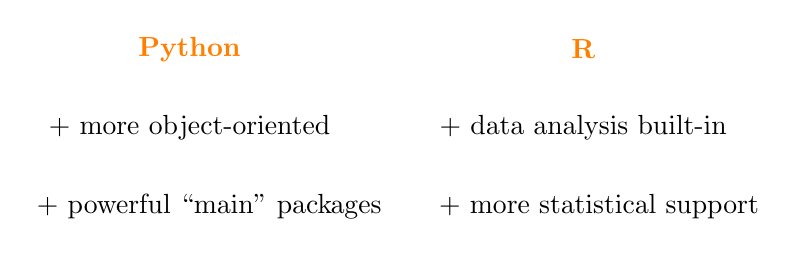
\begin{tikzpicture}
    \node[text=orange] (python) at (0, 0) {\textbf{Python}};
    \node[text=orange] (r) at (5, 0) {\textbf{R}};

    \node (python) at (0, -1) {+ more object-oriented};
    \node (python) at (0.25, -2) {+ powerful “main” packages};

    \node (python) at (5, -1) {+ data analysis built-in};
    \node (python) at (5.2, -2) {+ more statistical support};
    
\end{tikzpicture}
\end{document}